\documentclass{article}

\usepackage[utf8]{inputenc}
\usepackage[ngerman]{babel}
\usepackage{enumitem}
\usepackage{graphicx}
\usepackage{amsmath}
\usepackage{hyperref}
\usepackage{csquotes}

\newenvironment{auf}{Aufgabe}

\setlength{\parindent}{0cm}

\begin{document}
	\title{Klausurvorbereitung Physik}
	\author{Niklas Dießner}
	
	\maketitle
	\thispagestyle{empty}	
	\newpage
	
	\tableofcontents

	\section{Formelsammlung}
\subsection*{Gleichmäßig beschleunigte Bewegung}
Für die Geschwindigkeit $v$ in Abhängigkeit der Zeit $t$ mit einer konstanten Beschleunigung $a$ gilt:
\begin{align*}
    v=a\cdot t+v_0
\end{align*}
Für den Weg $s$ in Abhängigkeit der Zeit gilt:
\begin{align*}
    s=\frac{a}{2}\cdot t^2+v_0\cdot t+s_0
\end{align*}
Aus diesen beiden Gleichungen ergibt sich:
\begin{align*}
    v^2-v_0^2=2\cdot a\cdot s
\end{align*}
\subsection*{Elastischer Stoß}
Für zwei Körper mit den Massen $m_1$, $m_2$ und den Anfangsgeschwindigkeiten $v_1$, $v_2$ gilt:
\begin{align*}
    m_1\cdot v_1+m_2\cdot v_2=m_1\cdot v'_1+m_2\cdot v'_2
\end{align*}
\subsection*{Unelastischer Stoß}
Für zwei Körper mit den Massen $m_1$, $m_2$ und den Anfangsgeschwindigkeiten $v_1$, $v_2$ gilt:
\begin{align*}
    m_1\cdot v_1+m_2\cdot v_2=(m_1+m_2)\cdot u
\end{align*}
\subsection*{Drehmoment}
Greift an einem Körper eine Kraft $F$ an mit dem Abstand $r$ zum Schwerpunkt an entsteht folgendes Drehmoment $M$:
\begin{align*}
    M=r\cdot F
\end{align*}
Für einen Körper mit dem Drehmoment $M$, dem Trägheitsmoment $J$ und der Winkelbeschleunigung $\alpha$ gilt folgende Beziehung, welche auch als Grundgesetz der Dynamik bezeichnet wird.
\begin{align*}
    M=J\cdot \dot{\omega}=J\cdot \alpha
\end{align*}
\subsection*{Gegenüberstellung Translation Rotation}
\begin{center}
    \begin{tabular}{l l | l l}
        Translation & & Rotation & \\
        \hline
        Weg & $s$ & Drehwinkel & $\varphi$\\
        Geschwindigkeit & $v=\dot{s}$ & Winkelgeschwindigkeit & $\omega = \dot \varphi$\\
        Beschleunigung & $a=\dot{v}=\ddot{s}$ & Winkelbeschleunigung & $\alpha=\dot{\omega}=\ddot{\varphi}$\\
        Masse & $m$ & Trägheitsmoment & $J$\\
        Impuls & $p=m\cdot v$ & Drehimpuls & $L=J\cdot \omega$\\
        Kraft & $F=m\cdot a$ & Drehmoment & $M=J\cdot \alpha$\\
        Arbeit\footnotemark & $W=F\cdot s$ & Arbeit\footnotemark[1] & $W=M\cdot \varphi$\\
        Leistung\footnotemark[1] & $P=F\cdot v$ & Leistung\footnotemark[1] & $P=M\cdot\omega$\\
        kinetische Energie & $E_k=\frac{m}{2}v^2$ & Rotationsenergie & $E_k=\frac{J}{2}\omega^2$
    \end{tabular}
\end{center}
\footnotetext{Beziehungen gelten nur für einen speziellen Fall}
	
	\section{Mechanik der Punktmasse und des starren Körpers}
\begin{auf}
    154
\end{auf}
Eine mit Sand gefüllte Holzkiste der Masse $M=20kg$ ist an Schnüren der Länge $l=1.2m$ aufgehängt. In die anfangs ruhende Kiste wird ein Projektil der Masse $m=10g$ geschossen, wobei es in der Kiste stecken bleibt.
\begin{enumerate}
    \item[\ref{eq:154_a}] Welche Geschwindigkeit $v$ hatte das Projektil, wenn die Kiste dadurch maximal $x=4.9 cm$ horizontal ausgelenkt wird?
    \item[\ref{eq:154_b}] Wie groß ist der in Wärme und Verformungsarbeit umgewandelte Anteil der ursprünglich vorhandenen Energie?
\end{enumerate}
\begin{figure}[h]
    \centering
    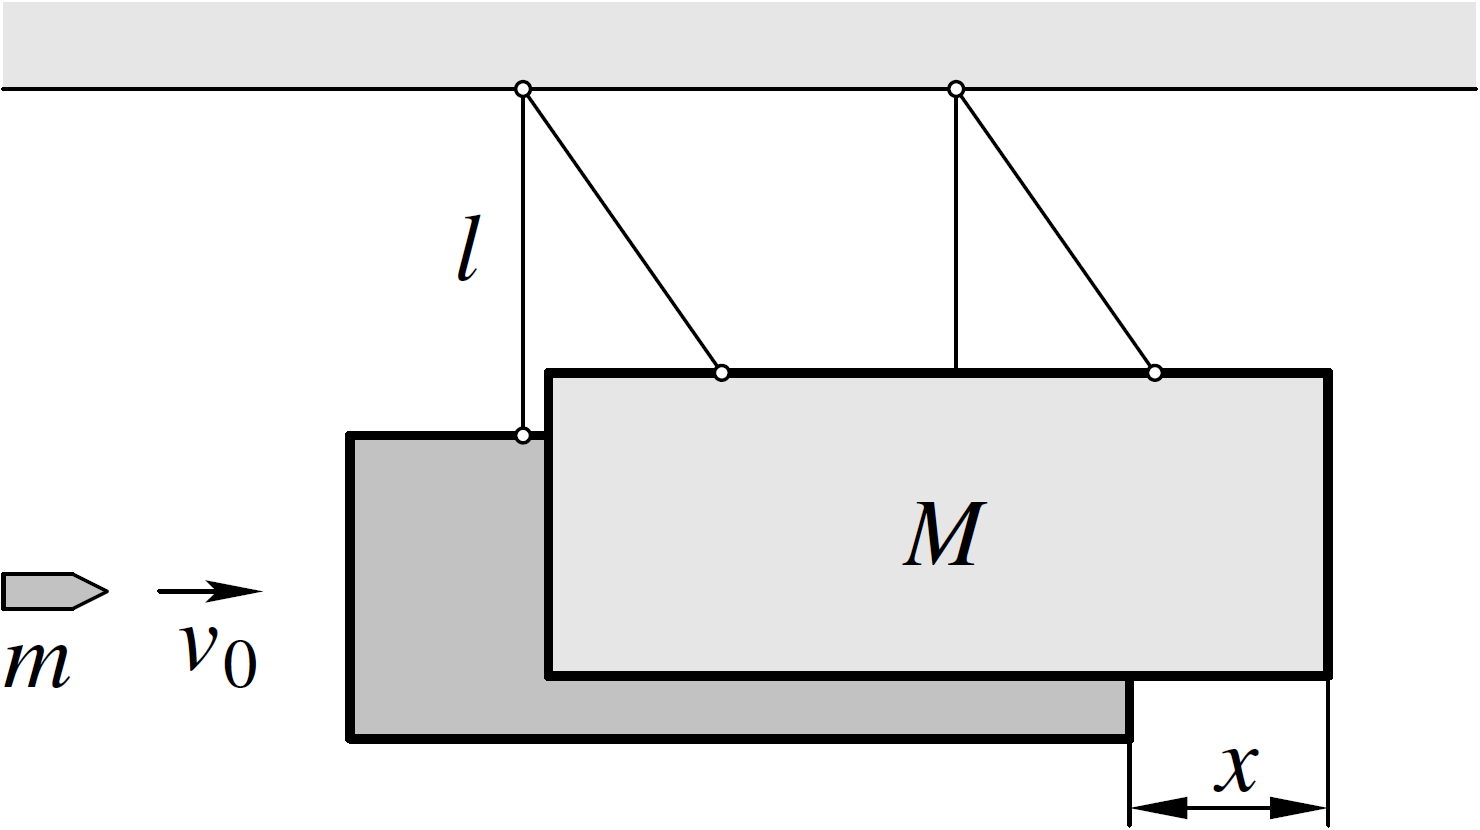
\includegraphics[width=0.7\linewidth]{images/154_0.png}
    \caption{Versuchsaufbau Aufgabe 154}
\end{figure}
Es handelt sich hierbei um einen unelastischen Stoß. Dabei hat die Masse $m$ zu Beginn die Geschwindigkeit $v$ und die Masse $M$ befindet sich anfangs in Ruhe, das heißt ihre Geschwindigkeit beträgt $0\frac{m}{s}$. Nach dem Stoß besitzen beide Massen die Geschwindigkeit $v'$.
\begin{align}
    m\cdot v &= (m+M)\cdot v'				\nonumber\\
    v&=\frac{m+M}{m}\cdot v' 				\nonumber\\
    v&=\left(1+\frac{M}{m}\right)\cdot v'	\label{eq:154_velocity0}
\end{align}
Bei der anschließenden Pendelbewegung vom hängenden Zustand 1 in den ausgelenkten Zustand 2 erfolgt eine Energieumwandlung von kinetischer Energie in potenzielle Energie. Es gilt der Energieerhaltungssatz. Dabei ist die potentielle Energie im Zustand 1 $0J$. Die kinetische Energie im Zustand 2 ist ebenfalls $0J$.
\begin{align}
    E_{kin_1}+E_{pot_1}&=E_{kin_2}+E_{pot_2}		\nonumber\\
    E_{kin_1}&=E_{pot_2}							\nonumber\\
    \frac{(m+M)\cdot v'^2}{2}&=(m+M)\cdot g\cdot h	\nonumber\\
    \frac{v'^2}{2}&=g\cdot h						\nonumber\\
    v'&=\sqrt{2\cdot g\cdot h}						\label{eq:154_velocity1}
\end{align}
Der Zusammenhang zwischen horizontaler und vertikaler Auslenkung ergibt sich aus dem Satz des Pythagoras.
\begin{figure}[h]
    \centering
    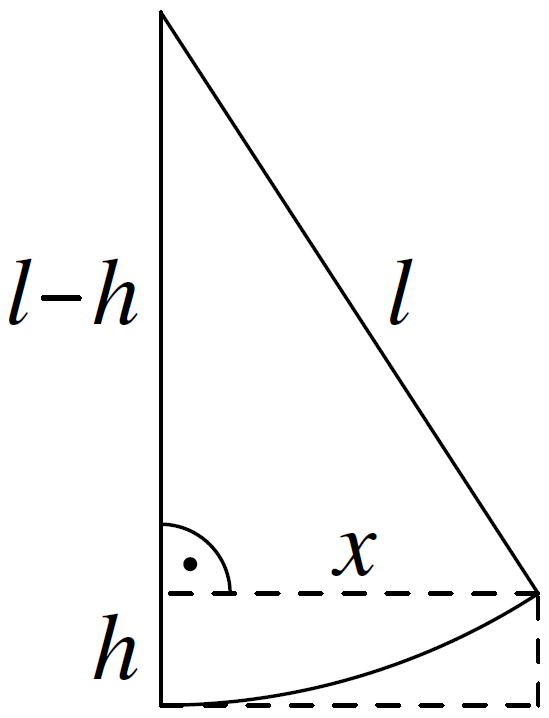
\includegraphics[height=2.5cm]{images/154_1.png}
    \caption{Skizze Pendelbewegung}
\end{figure}
\begin{align}
    (l-h)^2+x^2&=l^2		\nonumber\\
    (l-h)&=\sqrt{l^2-x^2}	\nonumber\\
    h&=l-\sqrt{l^2-x^2}		\label{eq:154_height}
\end{align}
Setzt man nun die Gleichungen \eqref{eq:154_height} und \eqref{eq:154_velocity1} in \eqref{eq:154_velocity0}, ein erhält man für die Anfangsgeschwindigkeit:
\begin{align*}
    v&=\left(1+\frac{M}{m}\right)\cdot\sqrt{2\cdot g\cdot\left(l-\sqrt{l^2-x^2}\right)}\\
    v&=\left(1+\frac{20kg}{0.01kg}\right)\cdot\sqrt{2\cdot 9.81\frac{m}{s^2}\cdot\left(1.2m-\sqrt{(1.2m)^2-(0.049m)^2}\right)}\\
    &\boxed{v=280.4\frac{m}{s}}		\tag{a} \label{eq:154_a}
\end{align*}
Um den Anteil der Energie, welcher in Wärme und Verformungsarbeit $\Delta E$ umgewandelt wurde, zu ermitteln sind die kinetische Energie vor und nach den Stoß zu betrachten. Dabei sei die Energie vor dem Stoß $E$.
\begin{align*}
    \Delta E&=\frac{m\cdot v^2}{2}-\frac{(m+M)\cdot v'^2}{2}\\
    \Delta E&=\frac{m\cdot v^2}{2}-\frac{m+M}{2}\cdot \left(\frac{m}{m+M}\cdot v\right)^2\\
    \Delta E&=\frac{m\cdot v^2}{2}-\frac{m^2\cdot v^2}{2\cdot(m+M)}\\
    \Delta E&=\left(1-\frac{m}{m+M}\right)\cdot\frac{m\cdot v^2}{2}\\
    \Delta E&=\left(1-\frac{m}{m+M}\right)E\\
    \Delta E&=\left(1-\frac{0.01kg}{0.01kg+20kg}\right)E\\
    &\boxed{\Delta E=0.9995E}		\tag{b}	\label{eq:154_b}
\end{align*}
	
	\begin{auf}
    204
\end{auf}
Eine Walze rollt frei hängend von einem Band ab, das auf ihren Umfang aufgewickelt ist und am oberen Ende festgehalten wird. Die Walze startet aus der Ruhelage und \enquote{durchfällt} eine Höhe von $h=2m$.
\begin{enumerate}
    \item[\ref{eq:204_a}] Wie groß ist ihre Beschleunigung?
    \item[\ref{eq:204_b}] Mit welcher Geschwindigkeit kommt sie unten an?
    \item[\ref{eq:204_c}] Welche Zeit benötigt sie dazu?
    \item[\ref{eq:204_d}] Wie verhält sich die Zugkraft des Bandes (Seilkraft) zur Gewichtskraft der Walze?
\end{enumerate}
\begin{figure}[h]
    \centering
    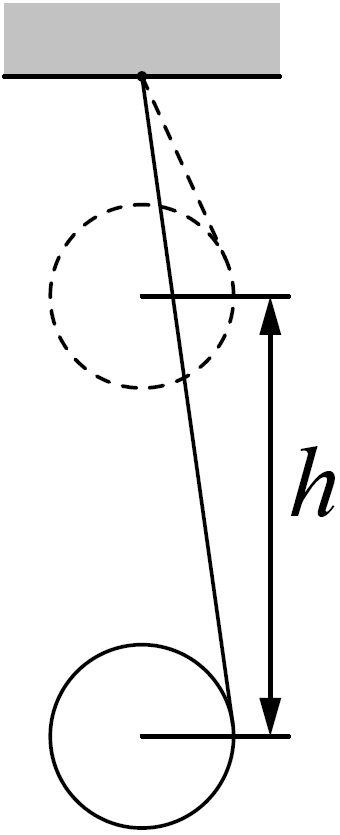
\includegraphics[height=5cm]{images/204_0.png}
    \caption{Versuchsaufbau Aufgabe 204}
\end{figure}
Die Kraft $F$, welche die Walze beschleunigt, ergibt sich aus der Seilkraft $F_S$ (nach oben) und der Gravitationskraft $F_G$ (nach unten).
\begin{align}
    F&=F_G-F_S					\nonumber\\
    m\cdot a &= m\cdot g - F_S	\nonumber\\
    F_S&=m\cdot(g-a)			\label{eq:204_force}
\end{align}
Die an der Walze anliegende Seilkraft erzeugt mit dem Radius $r$ der Walze ein Drehmoment $M$.
\begin{align}
    M=F_S\cdot r	\label{eq:204_torque0}
\end{align}
Für dieses gilt mit dem Trägheitsmoment $J$ und der Winkelbeschleunigung $\alpha$:
\begin{align}
    J&=\frac{m\cdot r^2}{2}			\nonumber\\
    \alpha&=\frac{a}{r}				\nonumber\\
    M&=J\cdot \alpha				\nonumber\\
    M&=\frac{m\cdot a\cdot r}{2}	\label{eq:204_torque1}
\end{align}
Setzt man nun \eqref{eq:204_force} in \eqref{eq:204_torque0} und die resultierende Gleichung mit \eqref{eq:204_torque1} gleich, erhält man:
\begin{align*}
    m\cdot(g-a)\cdot r&=\frac{m\cdot a\cdot r}{2}\\
    g-a&=\frac{a}{2}\\
    a&=\frac{2}{3}g\\
    &\boxed{a=6.54\frac{m}{s^2}}	\tag{a}\label{eq:204_a}
\end{align*}
Das Fallen der Walze ist eine gleichmäßig beschleunigte Bewegung. Dabei lässt sich folgende Aussage über das Verhältnis zwischen Start- und momentaner Geschwindigkeit treffen:
\begin{align*}
    v^2-v_0^2=2\cdot a\cdot s
\end{align*}
Da sich die Walze initial in Ruhelage befindet beträgt $v_0=0\frac{m}{s}$. Die zurückgelegte Strecke $s$ ist die Fallhöhe $h$.
\begin{align*}
    v^2&=2\cdot a\cdot h\\
    v&=\sqrt{2\cdot a\cdot h}\\
    v&=\sqrt{\frac{4\cdot g \cdot h}{3}}\\
    v&=\sqrt{\frac{4\cdot 9.81\frac{m}{s^2} \cdot 2m}{3}}\\
    &\boxed{v=5.11\frac{m}{s}}	\tag{b}	\label{eq:204_b}
\end{align*}
Da die Bewegung gleichmäßig beschleunigt ist, gilt dementsprechend:
\begin{align*}
    s&=\frac{a}{2}\cdot t^2+v_0\cdot t+s_0
\end{align*}
\newpage
Wie bereits erwähnt ist $s=h$ und die Anfangsgeschwindigkeit $v_0=0\frac{m}{s}$. Außerdem ist $s_0=0m$.
\begin{align*}
    h&=\frac{a}{2}\cdot t^2\\
    t^2&=\frac{2\cdot h}{a}\\
    t&=\sqrt{\frac{2\cdot h}{a}}\\
    t&=\sqrt{\frac{3\cdot h}{g}}\\
    t&=\sqrt{\frac{3\cdot 2m}{9.81\frac{m}{s^2}}}\\
    &\boxed{t=0.78s}	\tag{c}	\label{eq:204_c}
\end{align*}
Das Verhältnis von Zugkraft und Gewichtskraft ist beschrieben durch:
\begin{align*}
    \frac{F_S}{F_G}&=\frac{m\cdot(g-a)}{m\cdot g}\\
    \frac{F_S}{F_G}&=\frac{g-\frac{2}{3}g}{g}\\
    &\boxed{\frac{F_S}{F_G}=\frac{1}{3}}	\tag{d}	\label{eq:204_d}
\end{align*}
	
	\begin{auf}
    212
\end{auf}
Auf eine horizontal gelagerte Trommel (homogener Zylinder) der Masse $m=45.4kg$ ist ein Seil aufgewickelt, an dessen Ende eine Last von $m_1=10kg$ hängt (Ziehbrunnen).
\begin{enumerate}
    \item[\ref{eq:212_a}] Mit welcher Beschleunigung bewegt sich die Last aufgrund ihres Gewichts nach unten, wenn sich das Seil frei von der Trommel abwickelt? Reibung sowie Masse des Seiles werden vernachlässigt.
    \item[\ref{eq:212_b}] In welcher Zeit legt sie (beginnend aus der Ruhelage) eine Strecke von $20m$ zurück?
\end{enumerate}
\begin{figure}[h]
    \centering
    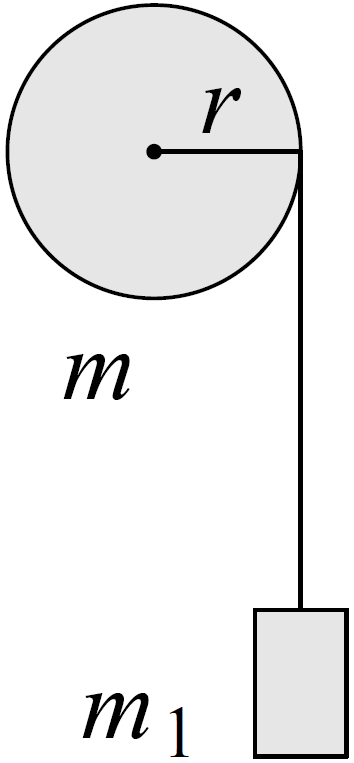
\includegraphics[height=5cm]{images/212_0.png}
    \caption{Versuchsaufbau Aufgabe 212}
\end{figure}
Die Gewichtskraft $F_G$ der Last zieht sie nach unten. Dieser wirkt die Seilkraft $F_S$ entgegen.
\begin{align}
    F&=F_G-F_S				\nonumber\\
    m_1\cdot a&=m_1\cdot g-F_S	\nonumber\\
    F_S&=m_1\cdot(g-a)	\label{eq:212_force}
\end{align}
Die Seilkraft erzeugt an der Trommel ein Drehmoment $M$.
\begin{align}
    M=F_s\cdot r	\label{eq:212_torque0}
\end{align}
Das Trägheitsmoment der Trommel $J=\frac{m\cdot r^2}{2}$, da es sich um einen Zylinder, welcher um seine Symmetrieachse rotiert. Die Winkelbeschleunigung ist ebenfalls bekannt mit $\alpha=\frac{a}{r}$.
\begin{align}
    M&=J\cdot\alpha	\nonumber\\
    M&=\frac{1}{2}\cdot m\cdot a\cdot r	\label{eq:212_torque1}
\end{align}
Man setzt \eqref{eq:212_torque0} und \eqref{eq:212_torque1} gleich. Dann setzt man \eqref{eq:212_force} ein.
\begin{align*}
    m_1\cdot(g-a)\cdot r&=\frac{1}{2}\cdot m\cdot a\cdot r\\
    m_1\cdot(g-a)&=\frac{1}{2}\cdot m\cdot a\\
    g-a&=\frac{m}{2m_1}\cdot a\\
    \frac{g}{a}-1&=\frac{m}{2m_1}\\
    \frac{g}{a}&=\frac{m+2m_1}{2m_1}\\
    a&=\frac{2m_1\cdot g}{m+2m_1}\\
    a&=\frac{2\cdot10kg\cdot9.81\frac{m}{s^2}}{45.4kg+2\cdot10kg}\\
    &\boxed{a=3\frac{m}{s^2}}	\tag{a}	\label{eq:212_a}
\end{align*}
Es handelt sich um eine gleichmäßig beschleunigte Bewegung. Das liefert den folgenden Ansatz. ($v_0=0\frac{m}{s}$, $s_0=0m$)
\begin{align*}
    s&=\frac{a}{2}t^2\\
    t^2&=\frac{2s}{a}\\
    t&=\sqrt{\frac{2s}{a}}\\
    t&=\sqrt{\frac{2\cdot20m}{3\frac{m}{s^2}}}\\
    &\boxed{t=3.65s}	\tag{b}	\label{eq:212_b}
\end{align*}
	
	\begin{auf}
    214
\end{auf}
Ein Vollzylinder vom Radius $R$ (Trägheitsmoment bezüglich der Zylinderachse $J_S =\frac{mR^2}{2}$) rollt aus der Ruhelage eine Strecke $s=2.5m$ auf der schiefen Ebene (Neigungswinkel $\alpha=20^\circ$) hinab.
\begin{enumerate}
    \item[\ref{eq:214_a}] Welche Geschwindigkeit hat der Zylinder unten?
    \item[\ref{eq:214_b}] Wie groß ist seine Beschleunigung und welche Zeit benötigt er für diese Strecke?
    \item[\ref{eq:214_c}] Welche Zeit benötigt im Vergleich dazu ein Hohlzylinder gleicher Masse, dessen Innenradius $r=\frac{9}{10}R$ beträgt? ($R$ Außenradius, Trägheitsmoment bezüglich der Zylinderachse $J_S=\frac{m(R^2 + r^2 )}{2}$.)
\end{enumerate}
\begin{figure}[h]
    \centering
    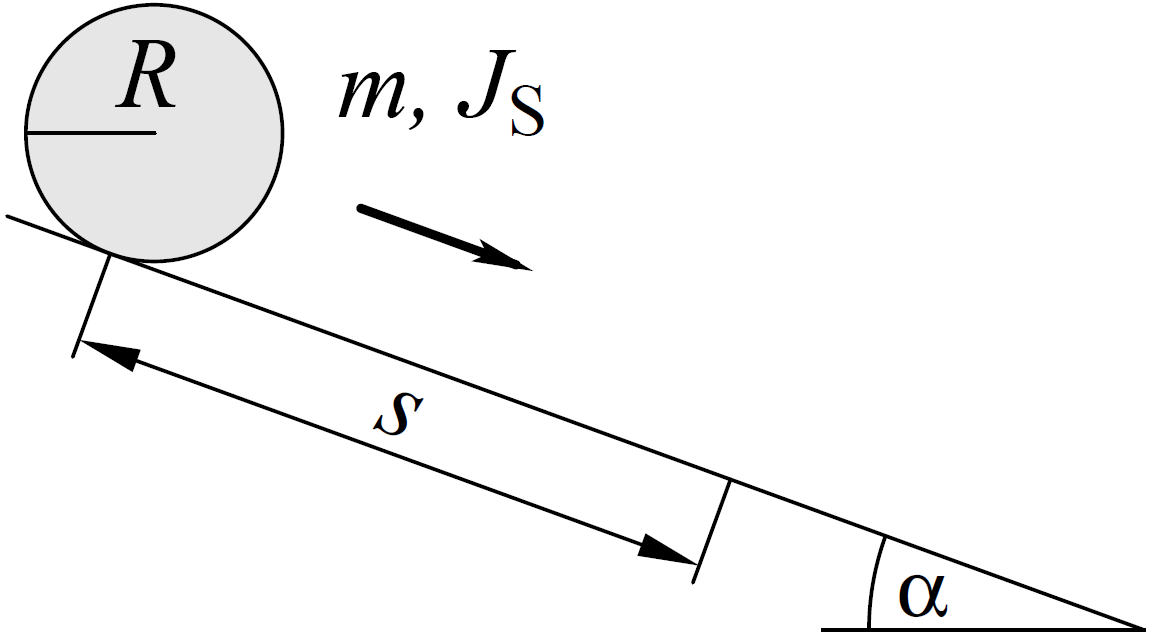
\includegraphics[width=0.7\linewidth]{images/214_0.png}
    \caption{Versuchsaufbau Aufgabe 214}
\end{figure}
Während des Herabrollen des Zylinders wird potentielle Energie $E_{Pot}$ in kinetische Energie $E_{Kin}$ und Rotationsenergie $E_{Rot}$ umgewandelt.
\begin{align*}
    E_{Pot}&=E_{kin}+E_{Rot}\\
    m\cdot g\cdot h&=\frac{m\cdot v^2}{2}+\frac{J_S\cdot\omega^2}{2}
\end{align*}
Dabei ist die Höhe $h=s\cdot\sin\alpha$, $J_S=\frac{m\cdot R^2}{2}$ und $\omega=\frac{v}{R}$.
\begin{align}
    m\cdot g\cdot s\cdot\sin\alpha&=\frac{m\cdot v^2}{2}+\frac{m\cdot R^2\cdot v^2}{4\cdot R^2}		\nonumber\\
    g\cdot s\cdot\sin\alpha&=\frac{v^2}{2}+\frac{v^2}{4}																		\nonumber\\
    g\cdot s\cdot\sin\alpha&=\frac{3}{4}v^2																								\nonumber\\
    v^2&=\frac{4\cdot g\cdot s\cdot\sin\alpha}{3}																						\nonumber\\
    v&=\sqrt{\frac{4\cdot g\cdot s\cdot\sin\alpha}{3}}																				\label{eq:214_velocity}\\
    v&=\sqrt{\frac{4\cdot 9.81\frac{m}{s^2}\cdot 2.5m\cdot\sin(20^\circ)}{3}}										\nonumber\\
    &\boxed{v=3.34\frac{m}{s}}	\tag{a}	\label{eq:214_a}
\end{align}
Es handelt sich um eine gleichmäßig beschleunigte Bewegung. Demnach gelten die folgenden Gleichungen.
\begin{align}
    v^2&=2\cdot a\cdot s	\nonumber\\
    a&=\frac{v^2}{2\cdot s}	\label{eq:214_acceleration}\\
    s&=\frac{a}{2}t^2		\nonumber\\
    t^2&=\frac{2s}{a}		\nonumber\\
    t&=\sqrt{\frac{2s}{a}}	\label{eq:214_time}
\end{align}
Man setzt \eqref{eq:214_velocity} in \eqref{eq:214_acceleration} ein. Im Anschluss setzt man diese Gleichung in \eqref{eq:214_time} ein.
\begin{align*}
    a&=\frac{\left(\sqrt{\frac{4\cdot g\cdot s\cdot\sin\alpha}{3}}\right)^2}{2\cdot s}\\
    a&=\frac{4\cdot g\cdot s\cdot\sin\alpha}{6\cdot s}\\
    a&=\frac{2\cdot g\cdot\sin\alpha}{3}\\
    t&=\sqrt{\frac{2s}{\frac{2\cdot g\cdot\sin\alpha}{3}}}\\
    t&=\sqrt{\frac{3s}{g\cdot\sin\alpha}}\\
    a&=\frac{2\cdot 9.81\frac{m}{s^2}\cdot\sin(20^\circ)}{3}\\
    t&=\sqrt{\frac{3\cdot2.5m}{9.81\frac{m}{s^2}\cdot\sin(20^\circ)}}\\
    &\boxed{a=2.24\frac{m}{s^2},\,t=1.50s}	\tag{b}	\label{eq:214_b}
\end{align*}
Für den Hohlzylinder bleibt die Ansatz der gleiche. Lediglich das Trägheitsmoment ändert sich.
\begin{align*}
    J_S&=\frac{m(R^2+r^2)}{2}\\
    r&=\frac{9}{10}R\\
    J_S&=\frac{m(R^2+\frac{81}{100}R^2)}{2}\\
    J_S&=\frac{181\cdot m\cdot R^2}{200}\\
    m\cdot g\cdot s\cdot\sin\alpha&=\frac{m\cdot v^2}{2}+\frac{181\cdot m\cdot R^2\cdot v^2}{400\cdot R^2}\\
    g\cdot s\cdot\sin\alpha&=\frac{v^2}{2}+\frac{181}{400}v^2\\
    g\cdot s\cdot\sin\alpha&=\frac{381}{400}v^2\\
    v&=\sqrt{\frac{400\cdot g\cdot s\cdot\sin\alpha}{381}}\\
    a&=\frac{\left(\sqrt{\frac{400\cdot g\cdot s\cdot\sin\alpha}{381}}\right)^2}{2\cdot s}\\
    a&=\frac{400\cdot g\cdot s\cdot\sin\alpha}{762\cdot s}\\
    a&=\frac{200\cdot g\cdot\sin\alpha}{381}\\
    t&=\sqrt{\frac{2s}{\frac{200\cdot g\cdot\sin\alpha}{381}}}\\
    t&=\sqrt{\frac{381s}{100\cdot g\cdot\sin\alpha}}\\
    t&=\sqrt{\frac{381\cdot2.5m}{100\cdot9.81\frac{m}{s^2}\cdot\sin(20^\circ)}}\\
    &\boxed{t=1.68s}	\tag{c}	\label{eq:214_c}
\end{align*}
	
	\section{Mechanik strömender Fluide}
\begin{auf}
    286
\end{auf}
Durch ein Rohr, bestehend aus zwei Teilstücken mit unterschiedlichem Querschnitt, die sich in verschiedenen Höhenlagen befinden, fließt Wasser (Dichte $\varrho=10^3\frac{kg}{m^3}$). Teilstück 1 hat den Durchmesser $D_1=9cm$, und der (statische) Druck in ihm beträgt $p_1=250kPa$. Im Teilstück 2 mit dem Durchmesser $D_2=20cm$, welches $\Delta h=15m$ höher liegt, soll der Druck $p_2=110kPa$ betragen.
\begin{enumerate}
    \item[a] Wie groß sind die Strömungsgeschwindigkeiten $v_1$ und $v_2$ in den beiden Teilstücken?
    \item[b] Wie groß sind Volumenstrom $I$ und Gesamtdruck $p_{ges}$ im Rohr?
\end{enumerate}
\begin{figure}[h]
    \centering
    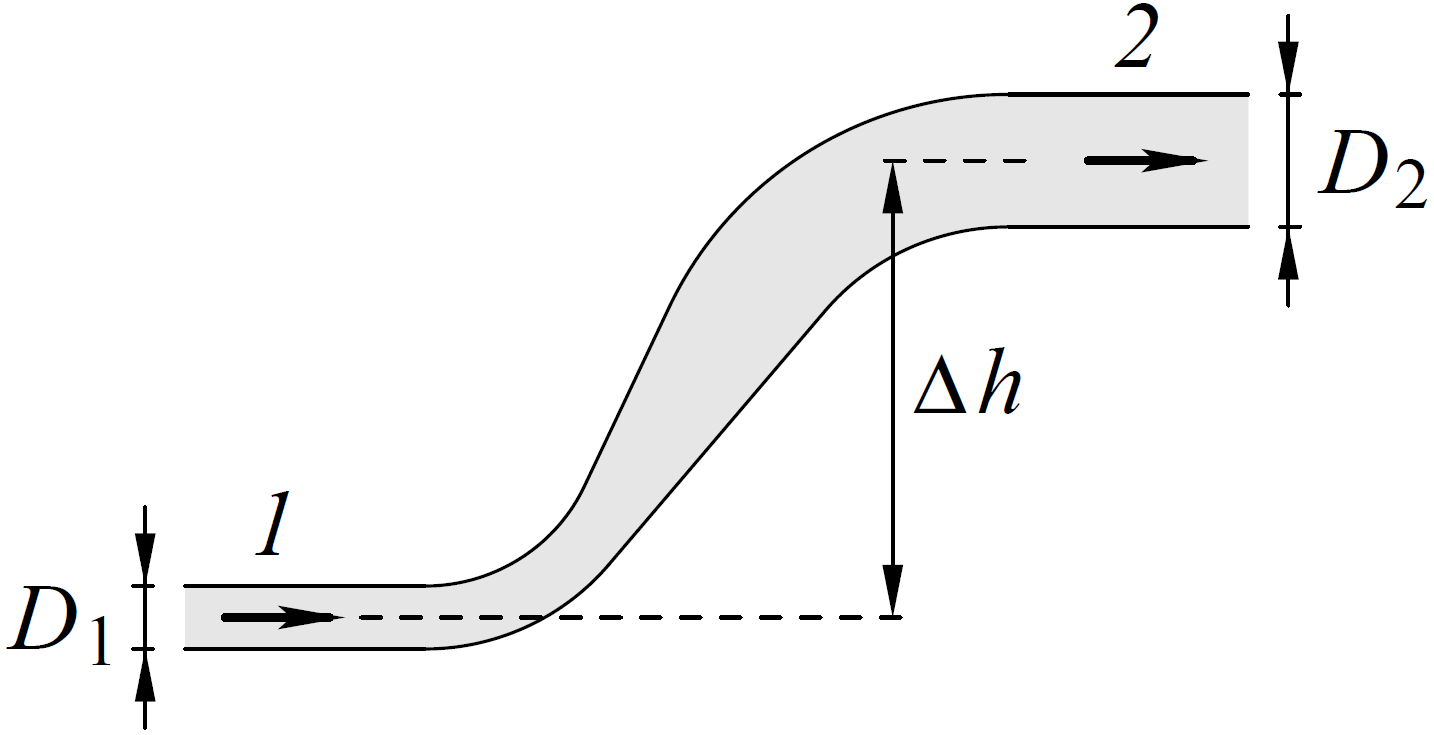
\includegraphics[width=0.7\linewidth]{images/286_0.png}
    \caption{Versuchsaufbau Aufgabe 286}
\end{figure}
Für beide Höhenniveaus $h_1=0$ und $h_2=\Delta h$ gilt die Bernoulli-Gleichung, wonach in beiden Teilstücken des Rohres der Gesamtdruck $p_{ges}$, das heißt die Summe aus statischem Druck (Kolbendruck) $p$, dynamischem Druck (Staudruck) $\frac{\varrho}{2}v^2$ und Schweredruck $\varrho\cdot g\cdot h$, gleich ist.
\begin{align}
    p_{ges}=p_1+\frac{\varrho}{2}v_1^2=p_2+\frac{\varrho}{2}v_2^2+\varrho\cdot g\cdot\Delta h	\label{eq:286_bernoulli}
\end{align}
Desweiteren gilt für die Volumenstromstärke $I$ in den beiden Querschnitten $A_1$ und $A_2$ die Kontinuitätsgleichung.
\begin{align}
    I=v_1\cdot A_1=v_2\cdot A_2	\label{}
\end{align}
	
	\begin{auf}
    287
\end{auf}
In ein strömendes Gewässer wird senkrecht von oben ein Staurohr so hineingehalten, dass der unter Wasser befindliche, im rechten Winkel gekrümmte Schenkel gegen die Strömung gerichtet ist. Das Wasser im Rohr steht um $\Delta h=10.0cm$ über der freien Wasseroberfläche. Wie groß ist die Strömungsgeschwindigkeit $v$?
\begin{figure}[h]
    \centering
    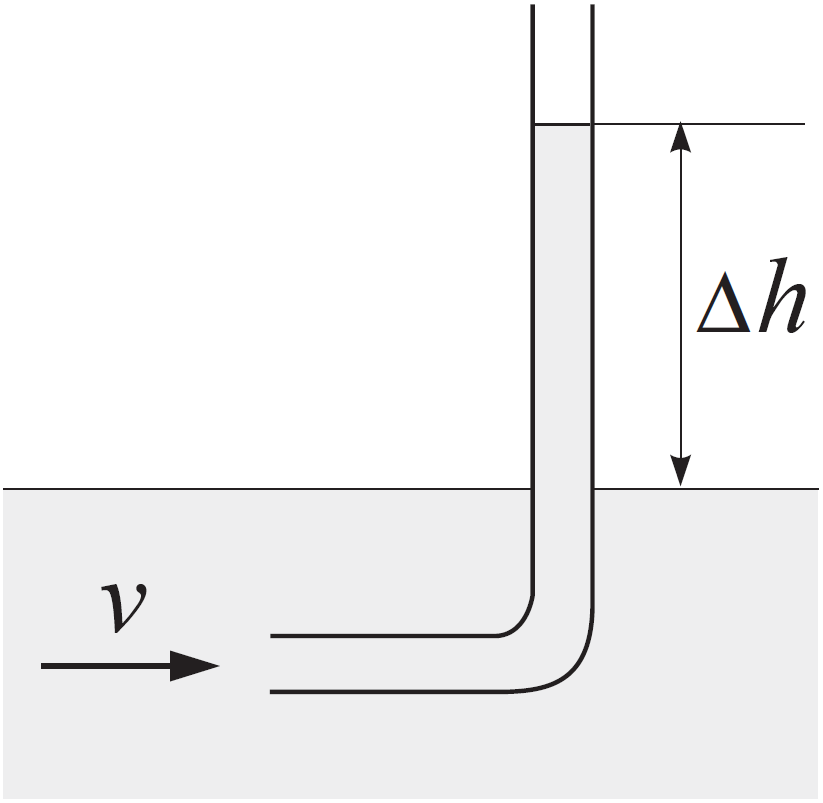
\includegraphics[height=5cm]{images/287_0.png}
    \caption{Versuchsaufbau Aufgabe 287}
\end{figure}
	
	\begin{auf}
    294
\end{auf}
Ein waagrechtes Rohr, das sich auf ein Drittel seines Durchmessers verjüngt, wird von Wasser ($\varrho = 10\frac{kg}{m^3}$) durchströmt. In den beiden unterschiedlich dicken Teilen des Rohres besteht eine (statische) Druckdifferenz von $6.4kPa$.
\begin{enumerate}
    \item[a] Wie groß sind die Strömungsgeschwindigkeiten in beiden Querschnitten?
    \item[b] Wie groß ist der Massenstrom $I_m$ für $D_1=12cm$ (Durchmesser des weiten Rohrteils)?
\end{enumerate}
	
	\begin{auf}
    295
\end{auf}
Bis zu welchem Druck $p_2$ kann der an den Ansaugstutzen (A) einer Wasserstrahlpumpe angeschlossene Rezipient evakuiert werden, wenn der bei 1 in das Strahlrohr vom Durchmesser 13 mm mit Leitungsdruck $p_1=3.2\cdot 10^5Pa$ eintretende Wasserstrahl an der Düse 2 auf den Durchmesser $5mm$ verengt wird, bevor er zusammen mit den aus dem Rezipienten angesaugten Luftmolekülen durch das dahinterliegende Auffangrohr wieder austritt? Der Volumenstrom des Wassers (Dichte $\varrho=10\frac{kg}{m^3}$) beträgt $0.5\frac{l}{s}$.
\begin{figure}[h]
    \centering
    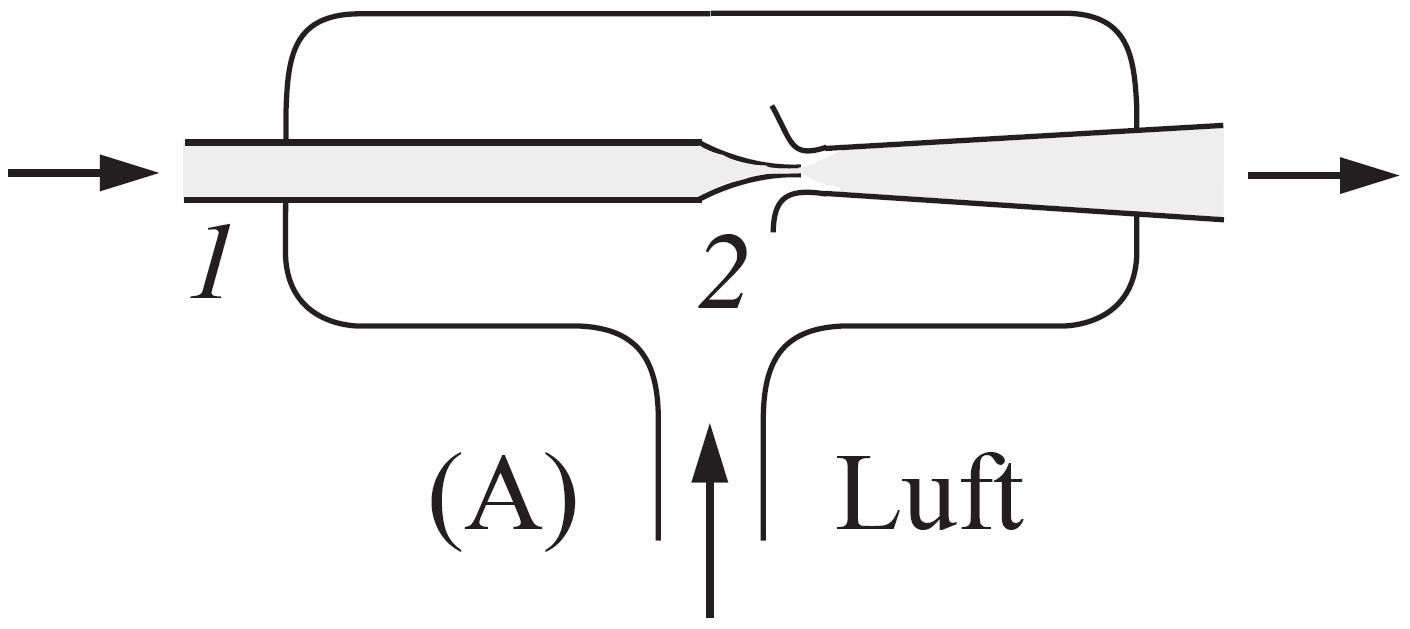
\includegraphics[width=0.7\linewidth]{images/295_0.png}
    \caption{Versuchsaufbau Aufgabe 295}
\end{figure}
	
	\section{Thermodynamik idealer Gase}
\begin{auf}
    360
\end{auf}
Luft vom Volumen $V_1=50cm^3$ und der Temperatur $T_1=300K$ soll bei konstantem Druck	von $p=1bar$ auf $T_2=1000K$ erwärmt werden.
\begin{enumerate}
    \item[a] Skizzieren Sie die Zustandsänderung in einem $p,V$-Diagramm.
    \item[b] Berechnen Sie das Endvolumen $V_2$.
    \item[c] Berechnen Sie die verrichtete Ausdehnungsarbeit $W_{12}$.
    \item[d] Berechnen Sie die Änderung der inneren Energie des Gases $\Delta U_{12}$, Adiabatenexponent $\kappa=\frac{c_p}{c_V}=1.4$
\end{enumerate}
	
	\begin{auf}
    362
\end{auf}
Luft (Molmasse $M\approx29\cdot10^{-3}\frac{kg}{mol}$) wird von einem Kompressor bei Atmosphärendruck $p_1=1bar$ und bei der Temperatur $T=294K$ angesaugt und auf den Druck $p_2=35bar$ verdichtet.
\begin{enumerate}
    \item[a] Wie groß ist die am Gas verrichtete Volumenarbeit je Kilogramm komprimierter Luft, wenn die Kompression isotherm erfolgen soll?
    \item[b] Welche Wärme $Q$ je Kilogramm Luft wird dabei an das Kühlwasser abgegeben?
\end{enumerate}
	
	\begin{auf}
    364
\end{auf}
Vom gleichen Anfangszustand 1 mit $p_1=1bar$, $V_1=1dm^3$ und $T_1=600K$ ausgehend expandiert ein Gas auf zwei verschiedenen Wegen zum gleichen	Endzustand 2 mit $V_2=2V_1$ und $T_2=\frac{T_1}{2}$. Der Weg 1-3-2 besteht aus einer Isotherme von 1 nach 3 und einer Isochore von 3 nach 2, der Weg 1-4-2 aus einer Isochore von 1 nach 4 und einer Isotherme von 4	nach 2. Wie groß sind auf beiden Wegen jeweils die verrichtete Arbeit $W$, die Änderung der inneren Energie des Gases $\Delta U$ und die ausgetauschte Wärme $Q$? $\kappa=1+\left(\frac{R_S}{c_v}\right)=1.4$.
\begin{figure}[h]
    \centering
    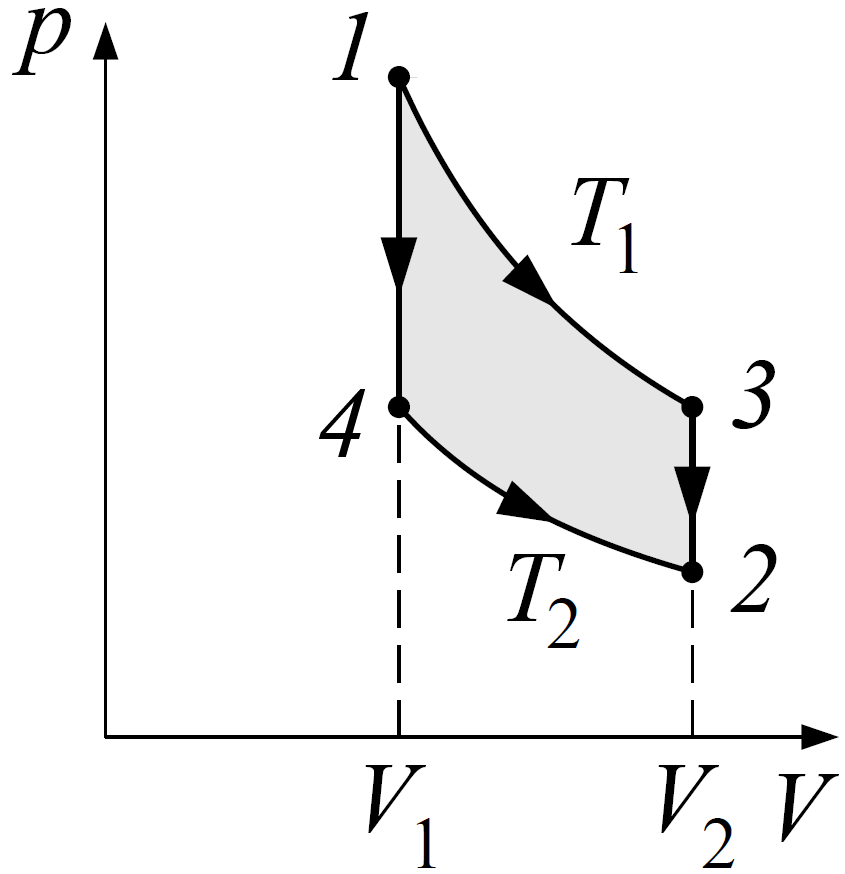
\includegraphics[height=5cm]{images/364_0.png}
    \caption{Versuchsaufbau Aufgabe 364}
\end{figure}
	
	\begin{auf}
    380
\end{auf}
Der im $V,T$-Diagramm dargestellte Kreisprozess wird von einem idealen Gas ($\kappa=\frac{c_p}{c_V}=1.67$) zwischen den Temperaturen $T_1$ und $T_2=\frac{T_1}{2}$ durchlaufen.
\begin{enumerate}
    \item[a] Man übertrage die Darstellung in ein $p,V$-Diagramm.
    \item[b] Berechnen Sie die zu- und abgeführten Wärmen auf allen drei Teilwegen sowie die Kreisprozessarbeit für $T_1=500K$, $V_1=5l$ und $p_1=1MPa$.
    \item[c] Wie groß ist der thermische Wirkungsgrad $\eta_{th}$ einer nach diesem Kreisprozess arbeitenden Wärmekraftmaschine?
\end{enumerate}
\begin{figure}[h]
    \centering
    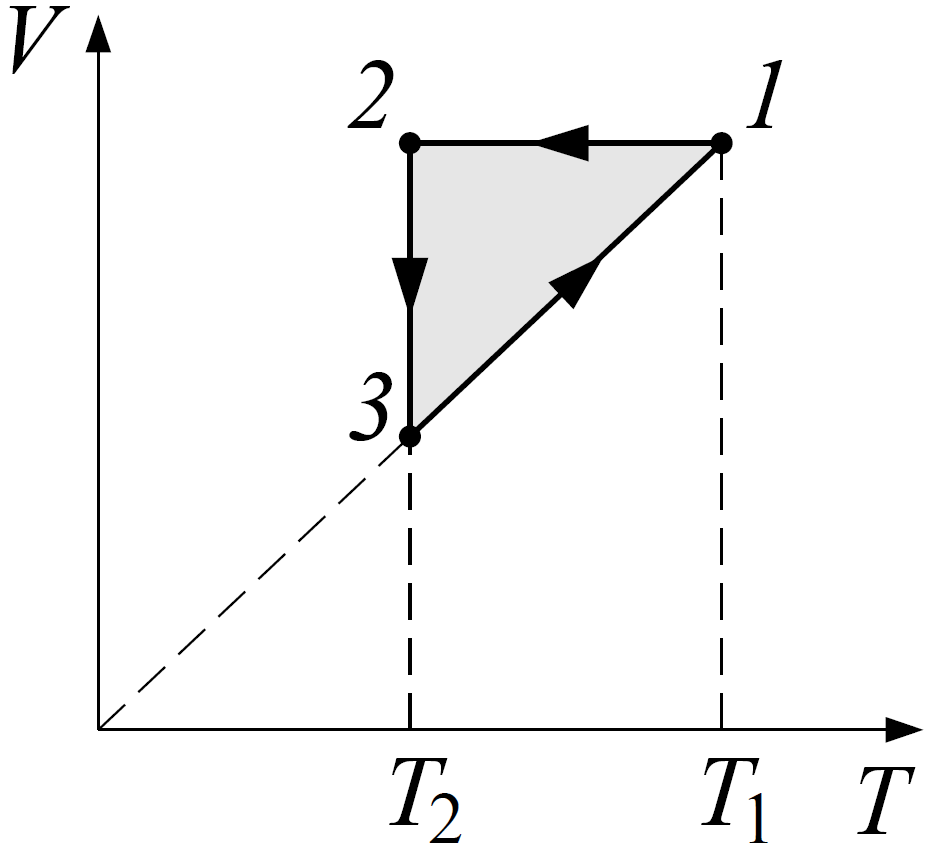
\includegraphics[height=5cm]{images/380_0.png}
    \caption{Versuchsaufbau Aufgabe 380}
\end{figure}
	
	\section{Elektrisches und magnetisches Feld}
\begin{auf}
    480
\end{auf}
Ein Elektron tritt senkrecht zu den elektrischen Feldlinien mit der Geschwindigkeit $v_0$ in den Vakuumraum eines Plattenkondensators ein und durchläuft ihn auf gekrümmter
Bahn.
\begin{enumerate}
    \item[a] Um welche Art von Bahnkurve handelt es sich?
    \item[b] Der Kondensator habe einen Plattenabstand von $d=4cm$ und eine Plattenlänge von $l=10cm$, die an den Platten anliegende Spannung ist $U=300V$. Mit welcher Geschwindigkeit	$v$ tritt das Elektron aus dem Kondensatorfeld aus, wenn $v_0=1.6\cdot10^7\frac{m}{s}$?
    \item[c] Wie groß ist die Abweichung $h$ von der ursprünglichen Bewegungsrichtung beim Austritt aus dem Feld?
    \item[d] Welche Änderung der Gesamtenergie erfährt das Elektron beim Durchqueren des Feldes?	Ladung des Elektrons $e=1.602\cdot10^{-19}C$, Masse des Elektrons $m=9.109\cdot10^{-31}kg$.
\end{enumerate}
\begin{figure}[h]
    \centering
    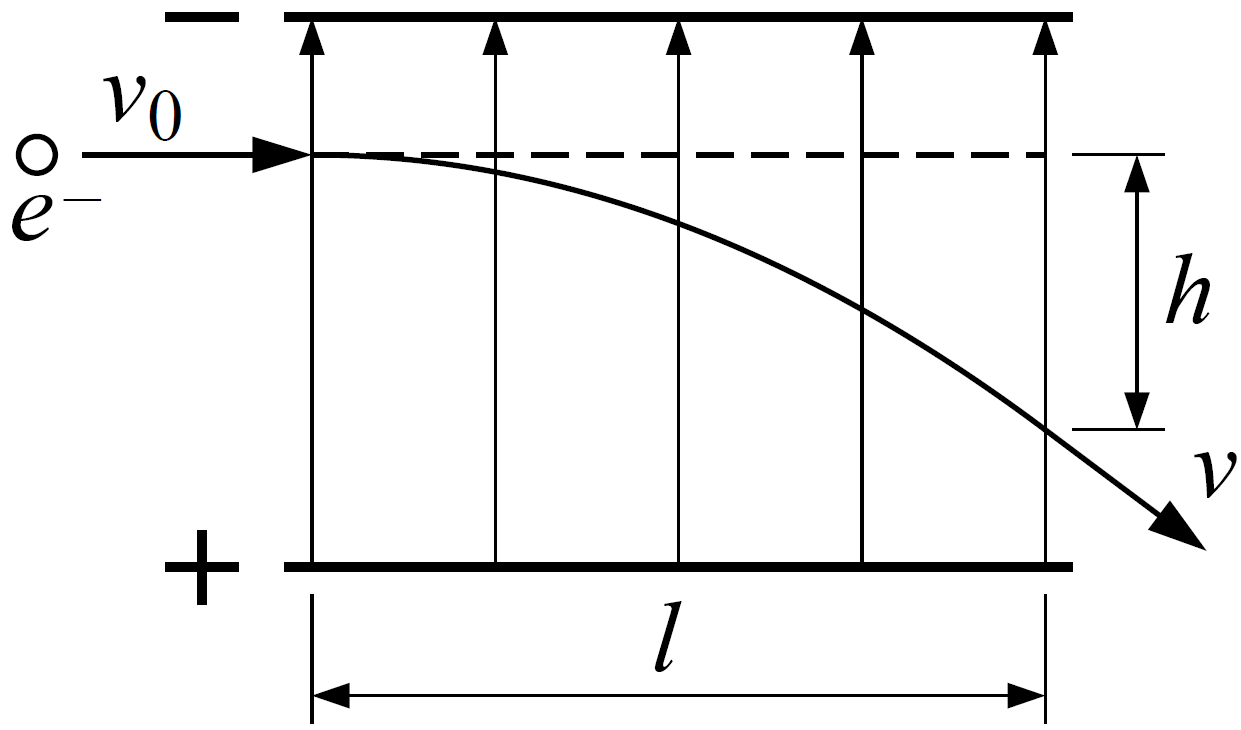
\includegraphics[width=0.7\linewidth]{images/480_0.png}
    \caption{Versuchsaufbau Aufgabe 480}
\end{figure}
	
	\begin{auf}
    508
\end{auf}
Ein Luftkondensator der Kapazität $C_0=80pF$ wird auf die Spannung $U_0=220V$ aufgeladen und danach
\begin{enumerate}
    \item[a] von der Spannungsquelle getrennt, 
    \item[b] an der Spannungsquelle belassen.	
\end{enumerate}
Wie ändern sich im Fall a und im Fall b Kapazität, Ladung, Spannung und Energieinhalt des Kondensators, wenn er mit Öl (Dielektrizitätszahl $\varepsilon_r=2,75$) gefüllt wird?
	
	\begin{auf}
    614
\end{auf}
Elektronen durchlaufen in einer Elektronenstrahlröhre zunächst eine Beschleunigungsspannung von $U=15kV$ und werden anschließend durch ein senkrecht zum Elektronenstrahl angeordnetes homogenes Magnetfeld von $B=8\cdot10^{-3}T$ abgelenkt. Die Anfangsgeschwindigkeit der Elektronen sei null, ihre spezifische Ladung beträgt $\frac{e}{m_e}=1.76\cdot10^{11}\frac{C}{kg}$.
\begin{enumerate}
    \item[a] Mit welcher Geschwindigkeit $v$ treten die Elektronen ins Magnetfeld ein?
    \item[b] Wie groß ist der Krümmungsradius $r$ der Bahn im Magnetfeld?
    \item[c] Mit welcher Geschwindigkeit $v_1$ treffen die Elektronen auf dem Leuchtschirm auf?
\end{enumerate}
\begin{figure}[h]
    \centering
    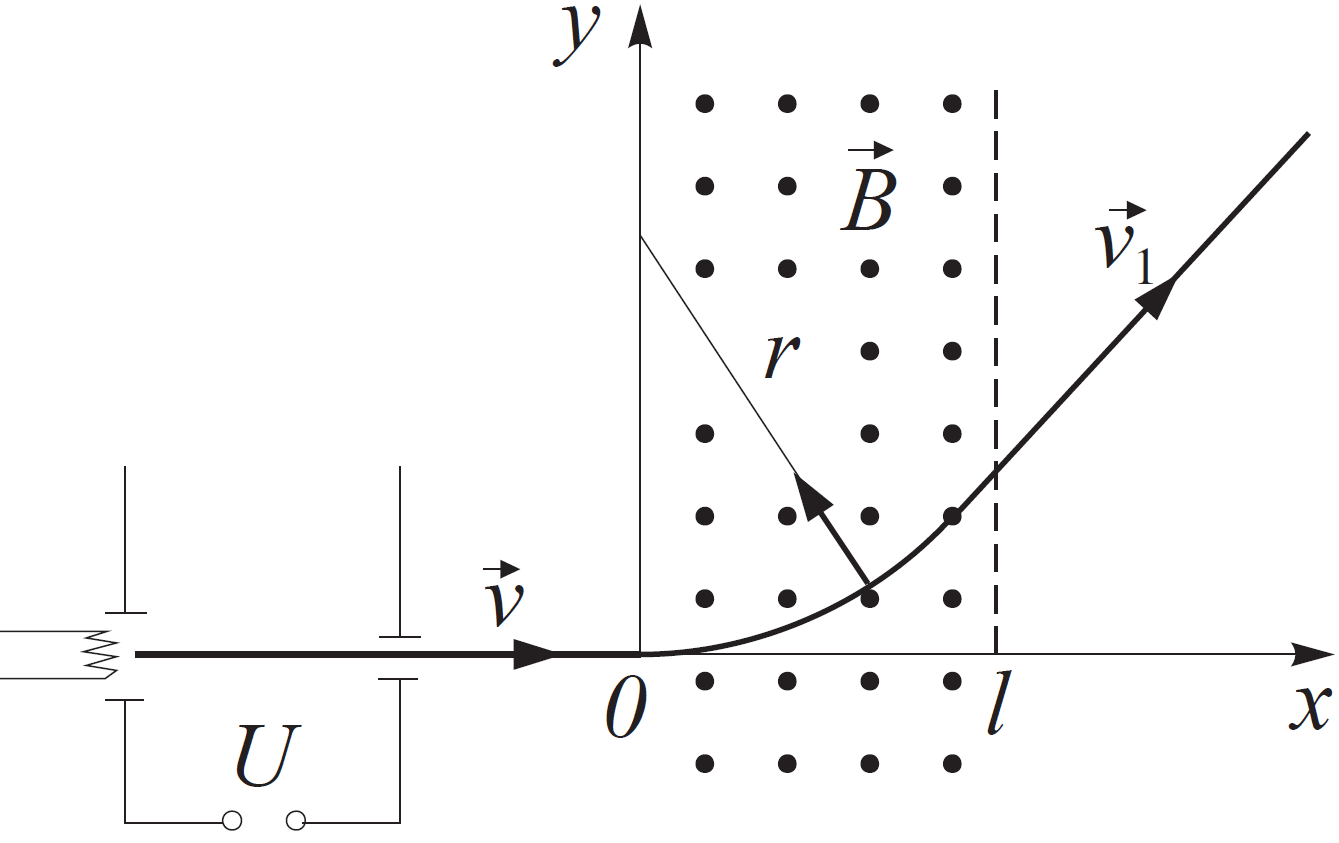
\includegraphics[width=0.7\linewidth]{images/614_0.png}
    \caption{Versuchsaufbau Aufgabe 614}
\end{figure}
	
	\begin{auf}
    620
\end{auf}
Zwischen den übereinander liegenden Polen eines Hufeisenmagneten befindet sich, an dünnen Stromzuführungen waagrecht aufgehängt, ein Draht aus Aluminium (Dichte $\varrho=2.7\cdot10\frac{kg}{m^3}$), welcher im vertikalen Magnetfeld (Flussdichte $B=0.08 T$) frei schwingen kann. Durch den Draht fließt ein Strom der Stromdichte $j=10^5\frac{A}{m^2}$. Um welchen Winkel $\varphi$ gegenüber der Senkrechten wird die Pendelaufhängung (sog. LORENTZ-Schaukel) ausgelenkt?
\begin{figure}[h]
    \centering
    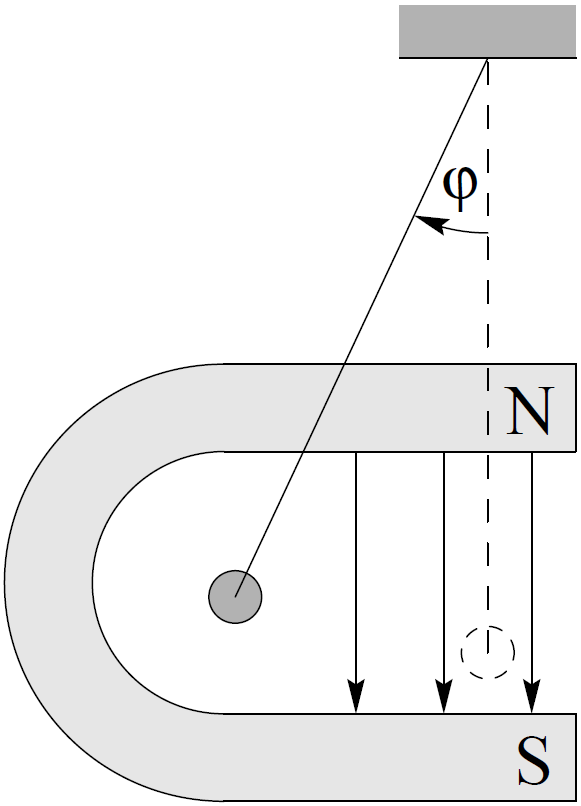
\includegraphics[height=5cm]{images/620_0.png}
    \caption{Versuchsaufbau Aufgabe 620}
\end{figure}
	
	\begin{auf}
    646
\end{auf}
Ein waagrechter, $l=40 mm$ langer und $d=2mm$ dicker runder Kupferstab tritt
frei fallend und beidseitig geführt durch zwei senkrechte, elektrisch leitende Schienen von vernachlässigbarem ohmschen Widerstand in ein horizontales homogenes
Magnetfeld der Flussdichte $B=0.035T$ ein und durchquert dieses.
\begin{enumerate}
    \item[a] Aus welcher Höhe $h$ über dem oberen Rand des Magnetfeldes muss der Stab losgelassen werden, wenn er das Feld mit konstanter Geschwindigkeit	$v$ passieren soll?
    \item[b] Wie groß sind betragsmäßig die induzierte Spannung, der Strom, die Bremskraft und die im Stab umgesetzte elektrische Leistung? In welcher Richtung fließt der Strom? Daten von	Kupfer: $\varrho_m=8.96\cdot10^3\frac{kg}{m^3}$, $\varrho=1.78\cdot10^{-8}\Omega m$.
\end{enumerate}
\begin{figure}[h]
    \centering
    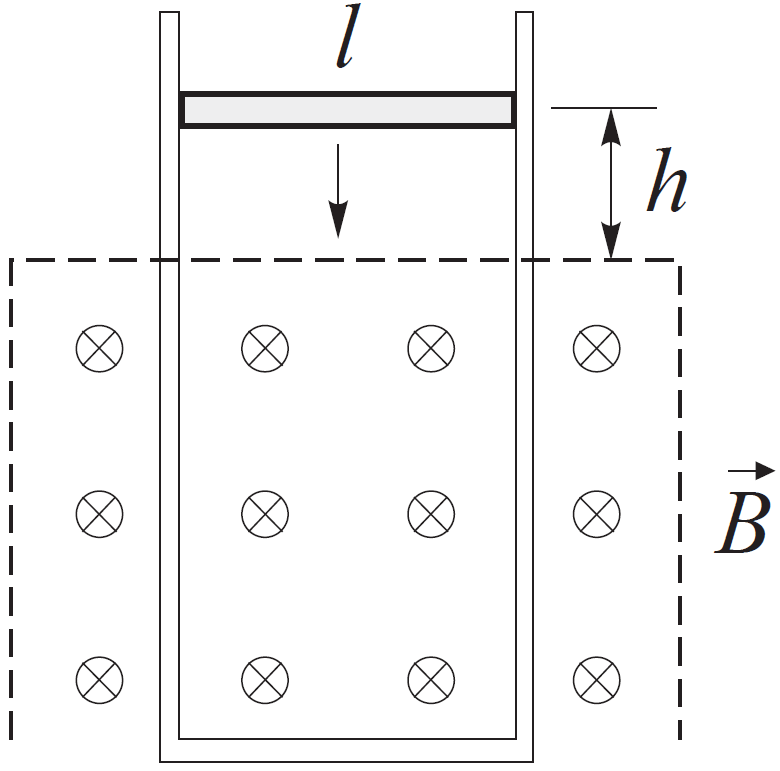
\includegraphics[height=5cm]{images/646_0.png}
    \caption{Versuchsaufbau Aufgabe 646}
\end{figure}
	
	\begin{auf}
    647
\end{auf}
Eine rechteckige Leiterschleife (Länge $l=8cm$, Breite $b=5cm$) befindet sich in einem homogenen Magnetfeld mit der Flussdichte $B=0.12T$.
\begin{enumerate}
    \item[a] Wie groß ist der magnetische Fluss $\Phi$ durch die Schleife, wenn \textbf{B} und die Flächennormale \textbf{A} einen Winkel von $30^\circ$ einschließen?
    \item[b] Wie groß ist die maximale induzierte Spannung, wenn die Schleife im Magnetfeld mit einer Winkelgeschwindigkeit von $\omega=100s^{-1}$ rotiert?
    \item[c] Welche Spannung wird induziert, wenn die Schleife so durch das Feld
    bewegt wird, dass \textbf{B} parallel zu \textbf{A} ist?
\end{enumerate}
\begin{figure}[h]
    \centering
    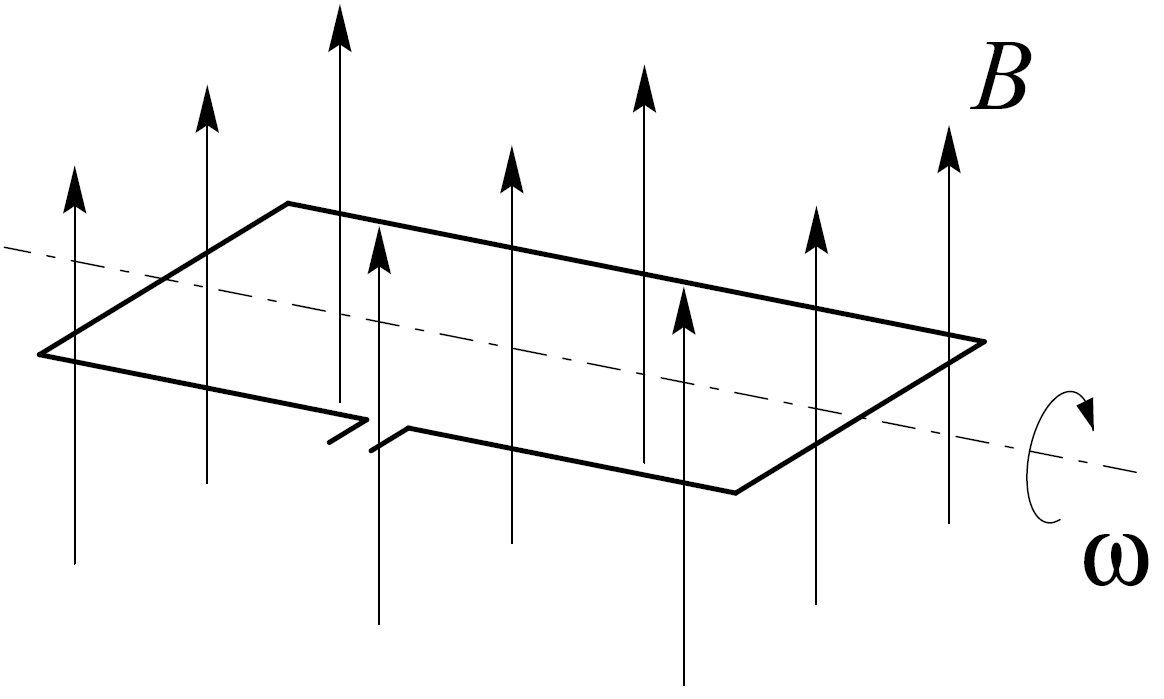
\includegraphics[width=0.7\linewidth]{images/647_0.png}
    \caption{Versuchsaufbau Aufgabe 647}
\end{figure}
	
	\section{Schwingungen und Wellen}
\begin{auf}
    683
\end{auf}
Senkrecht unter dem Aufhängepunkt A eines mathematischen Pendels der Pendellänge $l_1=1.0m$ befindet sich ein Stift S, an den sich der Pendelfaden beim Zurückschwingen anlegt (Pendelhemmung). Das Pendel schwingt dann nach rechts mit der verkürzten Pendellänge $l_2$.
\begin{enumerate}
    \item[a] Wie groß ist der Abstand des Stiftes vom Aufhängepunkt, wenn die Schwingungsdauer für beide Halbschwingungen zusammen $T=1.5s$ beträgt?
    \item[b] Wie hoch schwingt die Pendelmasse nach rechts aus, wenn das Pendel um $\varphi_1=3.0^\circ$ nach links ausgelenkt und	dann losgelassen wird?
    \item[c] Wie groß ist der maximale Auslenkungswinkel $\varphi_2$ beim Ausschwingen nach rechts?
\end{enumerate}
\begin{figure}[h]
    \centering
    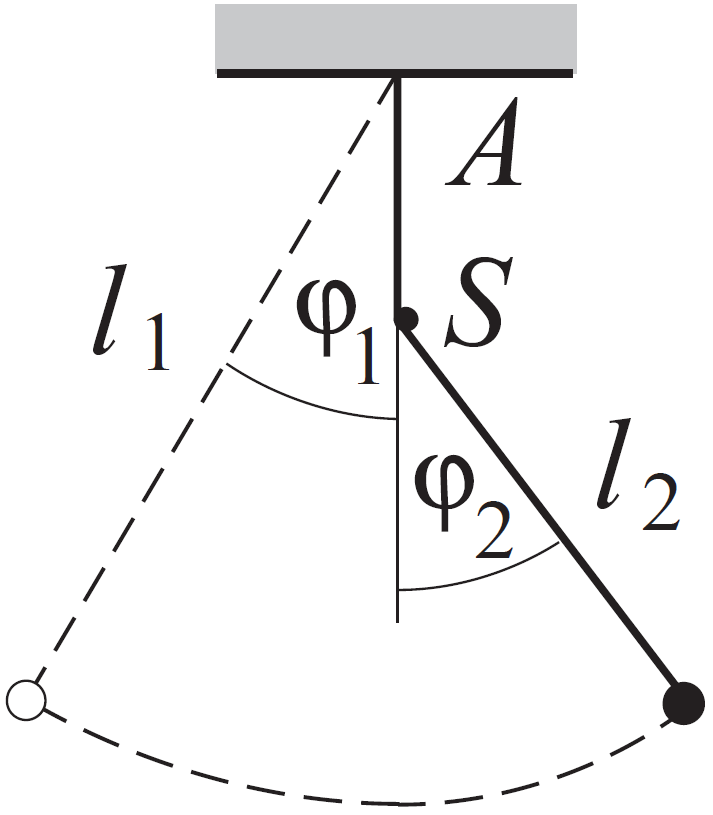
\includegraphics[height=5cm]{images/683_0.png}
    \caption{Versuchsaufbau Aufgabe 683}
\end{figure}
	
	\begin{auf}
    686.5
\end{auf}
Am Ende einer horizontal angeordneten Feder befindet sich eine Metallplatte von $m=0.1kg$ Masse. Die Feder wird, ausgehend von ihrer entspannten Ruhelage (1), um $x_m=5cm$ zusammengedrückt (2) und danach losgelassen. Reibung und die Gewichtskraft von $m$ werden vernachlässigt.
\begin{enumerate}
    \item[a] Wie lautet die Bewegungsgleichung (Differenzialgleichung) für die Masse $m$?
    \item[b] Wie groß ist die Federkonstante $k$, wenn die Platte harmonische Schwingungen mit der Periodendauer $T=0.5s$ ausführt?
    \item[c] Welche maximale Geschwindigkeit $v_m$ und maximale Beschleunigung $a_m$ erreicht die Platte	während der Schwingungen?
    \item[d] Skizzieren Sie die $x(t)$-, $v(t)$- und $a(t)$-Diagramme!
\end{enumerate}
\begin{figure}[h]
    \centering
    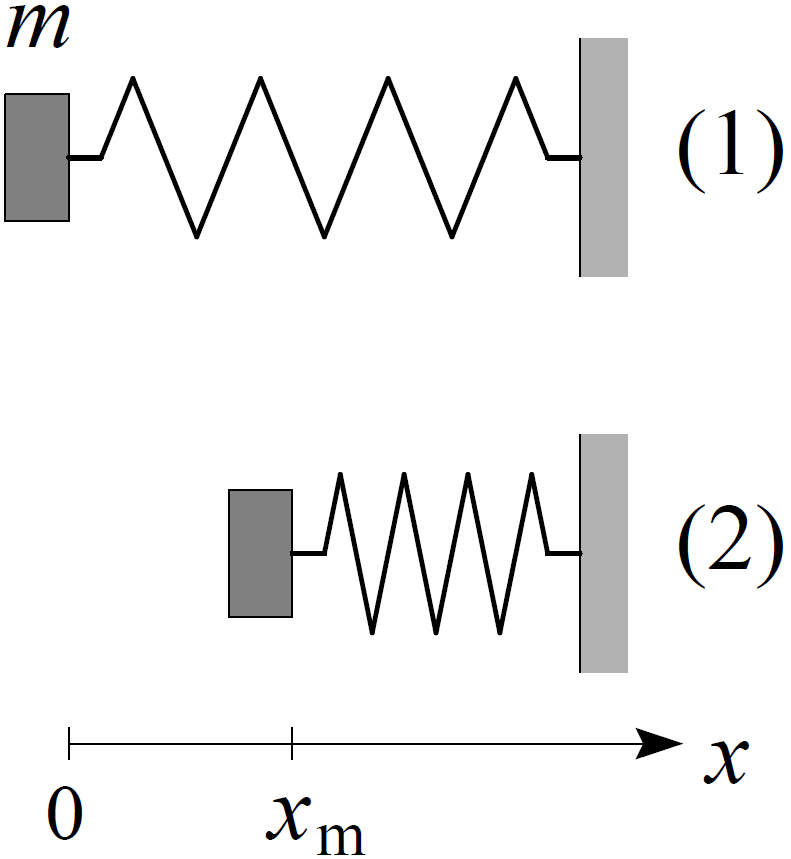
\includegraphics[height=5cm]{images/686,5_0.png}
    \caption{Versuchsaufbau Aufgabe 686.5}
\end{figure}
	
	\begin{auf}
    760
\end{auf}
Jemand befindet sich gleich weit von den beiden Lautsprechern einer Stereoanlage, die einen gegenseitigen Abstand von $d=4m$ haben, entfernt und hört einen reinen Ton. Er bewegt sich nun in seitliche Richtung um $x=0.5m$, bis der Ton wieder auf ein Lautstärkemaximum anschwillt.
\begin{enumerate}
    \item[a] Wie groß sind die Entfernungen $l_1$ und $l_2$ zu den Lautsprechern an diesem Ort?
    \item[b] Wie groß ist der Gangunterschied der eintreffenden	Schallwellen?
    \item[c] Welche Frequenz $f$ hat der Ton? Schallgeschwindigkeit	$340\frac{m}{s}$.
\end{enumerate}
\begin{figure}[h]
    \centering
    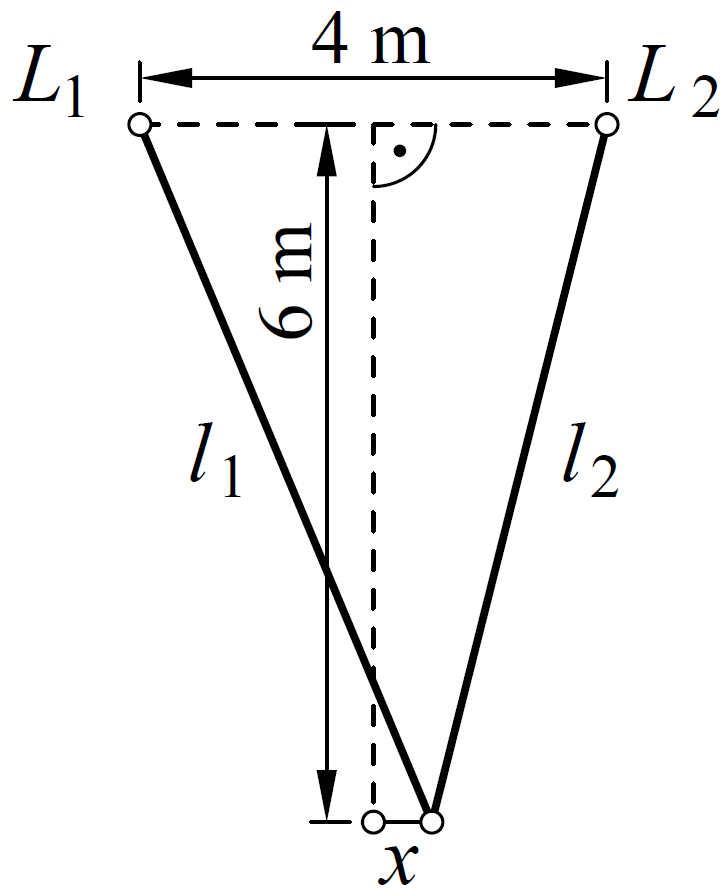
\includegraphics[height=5cm]{images/760_0.png}
    \caption{Versuchsaufbau Aufgabe 760}
\end{figure}
	
	\begin{auf}
    851
\end{auf}
Weißes Licht fällt aus der Luft kommend senkrecht auf eine Ölschicht (Dicke $d=0.7mm$; Brechzahl $n_2=1.5$), die sich auf einer Wasseroberfläche (Brechzahl $n_3=1.33$) ausgebreitet hat.
\begin{enumerate}
    \item[a] Wie groß ist der Gangunterschied zweier interferierender Wellen und an welcher	Grenzfläche tritt ein Phasensprung auf?
    \item[b] Wie lauten die Interferenzbedingungen für sich maximal verstärkende und sich gegenseitig auslöschende Lichtwellen?
    \item[c] Welche Wellenlängen werden im sichtbaren Bereich ($\lambda=380_{\cdots}780nm$) ausgelöscht?
\end{enumerate}
\begin{figure}[h]
    \centering
    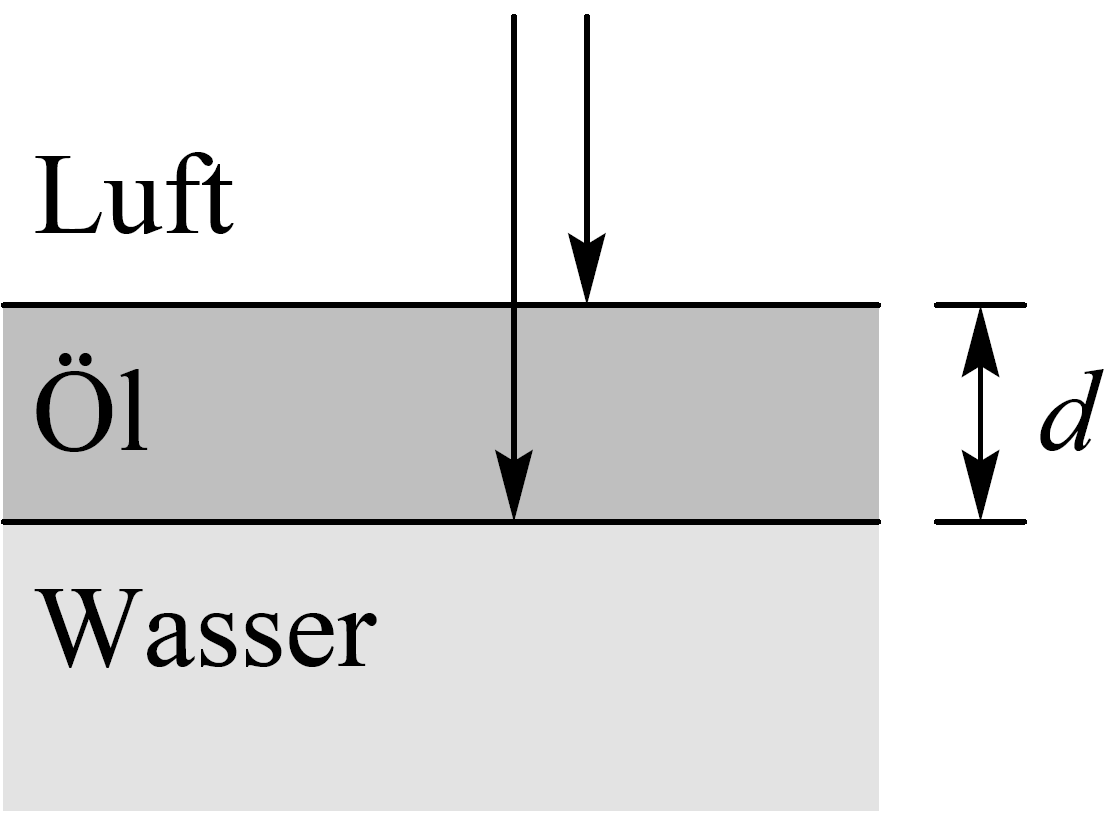
\includegraphics[height=5cm]{images/851_0.png}
    \caption{Versuchsaufbau Aufgabe 851}
\end{figure}
	
	\begin{auf}
		852
	\end{auf}
	Eine dünne plankonvexe Linse aus Glas ($n=1.5$) liegt mit der sphärisch gekrümmten Fläche auf einer ebenen Glasplatte. Die Linse wird senkrecht von oben mit monochromatischem Licht der Wellenlänge $\lambda$ beleuchtet. Mit einem Messmikroskop wird der Radius des dunklen NEWTONschen Ringes 1. Ordnung zu $r_1=840mm$, der Radius 5. Ordnung zu $r_5=1180mm$ ausgemessen (Blickrichtung von oben).
	\begin{enumerate}
		\item[a] An welchen	beiden Grenzflächen werden die interferierenden Strahlen reflektiert?
		\item[b] Wie groß ist $\lambda$, wenn der Krümmungsradius der Linse	$R=350mm$ beträgt?
		\item[c] Was beobachtet man im Zentrum, wenn die Linse exakt auf der Glasplatte aufliegt?
	\end{enumerate}
	\begin{figure}[h]
		\centering
		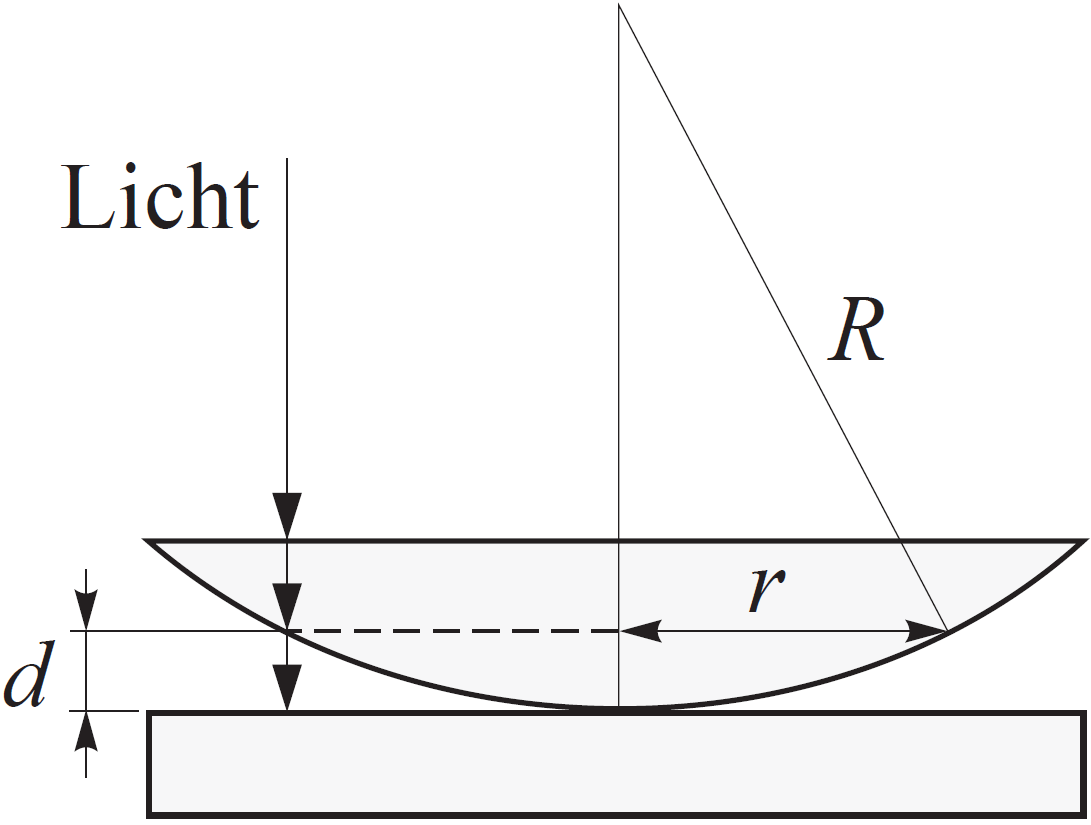
\includegraphics[height=5cm]{images/852_0.png}
		\caption{Versuchsaufbau Aufgabe 852}
	\end{figure}
\end{document}